\subsection{Python}
Python is the programming language used in the DAT110 course at UiS. Students are often struggling to understand how to work with objects because some objects are mutable and some are not. To make it easier for them to learn, a Python interpreter was implemented which parses a subset of the language. The interpreter returns an array of state objects, which contain information about the relationship between variables and objects after every statement. Together with the GraphDrawer, the interpreter can be used to ask questions about Python code. The student is able to see which object a variable points to, and they can see when the value or reference changes. Before the custom interpreter was implemented, using the official Python interpreter CPython \cite{CPython} was considered. Because of the size of CPython, and the limited time available for this project, it was decided that implementing a custom interpreter was the better option.
\\[11pt]
The following features of Python are supported:
\begin{enumerate}
    \item Variables of the following types: Number, String, Boolean, and Object. The Object type is any user-defined type.
    \item Functions can be defined using the \code{def} keyword. They can either belong to the global scope or a class. Functions can return something using the \code{return} keyword.
    \item Classes can be defined using the \code{class} keyword. If a function with the \code{\_\_init\_\_} name is defined inside the class, it will be called when a new instance of the class is instantiated.
    \item IF statements can be created with the \code{if} keyword. ELIF and ELSE statements are also supported.
    \item The following mathematical operators are supported: +, -, /, *.
    \item The following comparison operators are supported: and, or, !, ==, !=, <, >, >=, <=.
    \item Expressions can be grouped and separated using parentheses.
    \item Lines starting with a \# are treated as comments and will be skipped by the interpreter.
\end{enumerate}
Significant Python features missing from this interpreter:
\begin{enumerate}
    \item The standard library.
    \item Lists and dictionaries.
    \item Inner classes and functions.
    \item Shared class variables.
    \item Class inheritance.
    \item Loops.
\end{enumerate}
Every operator has the same priority, which means that expressions are always evaluated left to right. This makes some expression behave in an unexpected way. The following statement results in an error: \code{if 1 + 1 == 2:}, because it is evaluated as \code{1 + (1 == 2)}. To prevent this from happening, parentheses should be used to separate the expressions. The correct statement would be: \code{if (1 + 1) == 2:}.

\subsubsection{Interpreter}
There are three main functions in the interpreter. \code{parseLine} tries to figure out what the meaning of a code line is. \code{parseLine} is also responsible for deciding which line to parse next. A line can either be a variable assignment which is handled by the \code{parseLine} function, an expression which is handled by the \code{evaluateExpression} function, or a statement which is handled by the \code{handleKeyword} function. A statement is anything starting with one of the keywords. An expression is something which can be evaluated to a value.
\begin{figure}[H]
    \centering
    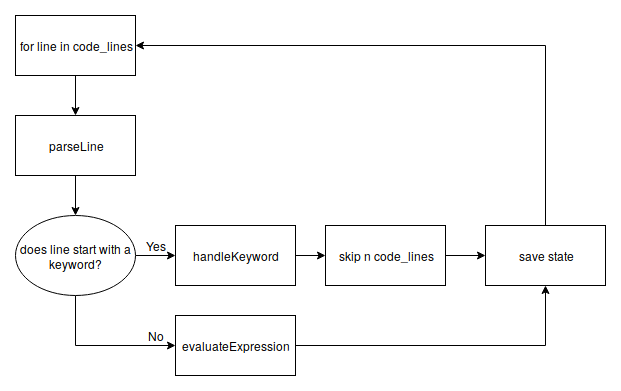
\includegraphics[width=0.75\linewidth]{/python/codelinepath}
    \caption{Interpreter loop}
    \label{fig:pythonCodeLinePath}
\end{figure}
\noindent
An important feature of the interpreter is the scope objects. A scope is an object with information about the variables, classes, functions, and data inside the scope. Functions are scopes because they can contain private variables. Classes are also scopes because they can contain functions. Before code can be parsed, a global scope is created. Anything not belonging to a specific scope is placed in the global scope. Scope data is an array where the index is the address of the stored data and the value is the stored data. Because the interpreter is implemented in JavaScript, there is no need to separate value and references types in this array, because JavaScript and Python behave the same way. Scope variables are a mapping from variable names to data addresses. Scope functions/classes are mappings from function/class names to function/class objects. Because the interpreter should save the state of the program as steps, the \code{parseLine} function returns an object containing information about the state. If the state was anything other than a function or class definition, the current state is saved as a step.
\\[11pt]
A function is an object with a \code{name}, a list of arguments \code{args}, a list of the code lines belonging to the function \code{code}. A function should also be a scope. The name is used to identify the function. The arguments are used to make sure that when the function is called, the right amount of arguments are passed. The code is stored so the function can be evaluated when it is called. After a function has been defined, the \code{handleKeyword} function returns a state of type \code{"SkipLines"} which tells the caller which lines have already been handled. The interpreter uses the \code{callFunc} function to call Python functions. When a function is called, three things happen in the following order:
\begin{enumerate}
    \item The function arguments are added as local variables. Local variables mean they belong to the function scope. The arguments need to be in the same order as they were defined because named arguments are not implemented.
    \item Every line found in the functions \code{code} list is parsed using \code{parseLine}. If a \code{return} statement is found before reaching the end, the function will stop parsing, before reaching the end.
    \item The scope of the function is restored to an empty state and data is returned if a return statement was found.
\end{enumerate}
A class is an object with a \code{name} and a list of the code lines belonging to the class \code{code}. A class should also be a scope. When a class is defined, the code is also parsed using the \code{parseLine} function. This is done so that any functions within the class is defined in the scope of the class. When the interpreter is instantiating an instance of the class, the \code{instantiateClass} function is called. \code{instantiateClass} first creates a new object containing all the functions from the class. If the class has a constructor it is called. Finally, the object is returned to the caller of \code{instantiateClass}.
\\[11pt]
When a code line is not a statement, it is passed to \code{evaluateExpression} so that it can be parsed. The following list contains information about how the parser determines what kind of expression the line is, and in what order, it happens.
\begin{enumerate}
    \item The function starts by checking if the line is a base type value. Base types are defined as String, Number, and Boolean. If the expression is determined to be a base type value, an object containing the \code{type} and \code{value} is returned. 
    \item If the expression is not a base type value, then it could be a variable. The current scope is checked to see if it contains a variable with the same name as the line. If it does, the data referenced by the variable is returned.
    \item If the line contains a "." it could be a property access or a function call. The possible object and property names are extracted. If an object with the given property name exists, the referenced data is returned. If it does not exist, the expression can either be an undefined property, or an operation, e.g. \code{self.x + 1} will first evaluate to the property \code{x + 1} of the \code{self} object. If the property is undefined, an error will be thrown. If the property name contains an operation, it can be resolved by evaluating the \code{propertyName} as an expression relative to the object scope.
    \item The expression is now checked if it is an operation, function call or class instantiation. This is done by looking at the parentheses.
    \item If the expression is a function call or a class instantiation, the arguments are extracted and evaluated, before the function is called. This is done because a function call can contain expressions inside it, and any argument which is not an expression will return itself. Example: This \code{my\_console.print("Hello, " + "World! From: " + my\_name)} function call contains one argument call referencing variables belonging to the global scope. When the function is called, the code is evaluated relative to the \code{my\_console} scope, which does not contain a reference to the \code{my\_name} variable. Python does not allow classes and functions to have the same name, meaning that there is no need to differentiate between function calls and class instantiation, because class instantiation is a function call to the \code{\_\_init\_\_} function.
    \item Any expression which has not already been evaluated should be an operation. An operation is an expression containing at least one operator and at least one expression. An operation expression is always evaluated left to right unless parentheses are used to group and separate operations. E.g. \code{1 + 2 + 3} is split into expression1 = 1, operator = + and expression2 = "2 + 3".
\end{enumerate}
Python code is always written on the client side by a user and then sent to the server so it can be interpreted. Code is simply text, so transferring it works flawlessly. After the code has been parsed, it is either stored in the database when a question is created or sent back to the user if it came from the sandbox. The result of the interpretation is an array of state objects. Normally one of the state objects could be inspected, and it would be possible to see that both \code{a} and \code{b} reference the same object in the following code snippet:
\code{
    a = "Dummy-text"
    b = a
}.
Before transferring a JavaScript object to a database or over a network, the object needs to be converted to a JSON object. When this conversion happens, the references are lost. They are also not available when the JSON object is converted back to a JavaScript object. When inspecting the code, it would like \code{a} and \code{b} reference two different objects with the same value. For this reason, a system for manually tracking object references was implemented. Every scope, variable and object is assigned a unique id. When the SolutionChecker or the GraphDrawer wants to check if two objects are the same, the usual JavaScript comparison (\code{a == b}) cannot be used because it would always return false. Instead, the id needs to be checked, \code{a.id == b.id}. The id stays the same between different interpretation steps, and this means that the GraphDrawer can keep track of which variable links to what object simply by creating a mapping from the unique id to the GraphDrawer node.
